 
\section{Problem 1}
\label{part1}
\begin{verbatim}
We know the result of the Karate Club (Zachary, 1977) split.
Prove or disprove that the result of split could have been predicted
by the weighted graph of social interactions.  How well does the
mathematical model represent reality?

Generously document your answer with all supporting equations, code,
graphs, arguments, etc.

Useful sources include:

* Original paper

http://aris.ss.uci.edu/~lin/76.pdf

* Slides

http://www-personal.umich.edu/~ladamic/courses/networks/si614w06/ppt/lecture18.ppt

http://clair.si.umich.edu/si767/papers/Week03/Community/CommunityDetection.pptx

* Code and data

http://networkx.github.io/documentation/latest/examples/graph/karate_club.html

http://nbviewer.ipython.org/url/courses.cit.cornell.edu/info6010/resources/11notes.ipynb

http://stackoverflow.com/questions/9471906/what-are-the-differences-between-
community-detection-algorithms-in-igraph/9478989#9478989

http://stackoverflow.com/questions/5822265/are-there-implementations-of
-algorithms-for-community-detection-in-graphs

http://konect.uni-koblenz.de/networks/ucidata-zachary

http://vlado.fmf.uni-lj.si/pub/networks/data/ucinet/ucidata.htm#zachary

https://snap.stanford.edu/snappy/doc/reference/CommunityGirvanNewman.html

http://igraph.org/python/doc/igraph-pysrc.html#Graph.community_edge_betweenness

\end{verbatim}

\subsection{Solution}

\begin{enumerate}
\item Karate club got split into two groups after the dispute.
\item I now implemented Girvan-Newman Algorithm which uses edge betweenness to split a group into sub groups.
\item Edge betweenness is defined as the number of times that a particular edge is used by every node to connect all other nodes. 
\item Now using the concept of Girvan-Newman Algorithm, I need to find out the maximum edge betweenness among all the edges.
\item The edge that has the maximum edge betweenness is deleted.
\item This process is continued till a new group or cluster is formed.
\item Now In order to do this I got the karate club data in GraphML format. This can be seen in figure\ref{g1}.
\item In order to plot the graph and calculate the edge betweenness, I found out that a library called ``igraph'' can be used.
\item I tried to install igraph library in my laptop which has windows operating system, but it did not work out.
\item So, I went on to install igraph on mac but I got an error with ``cairo'' library. 
\item Later on I figured out that it was working fine in ubuntu. 
\item I wrote a python code to calculate edge with maximum edge betweenness and deleted it each time in a loop. Code can be seen in listing\ref{lst:q1-1}
\item This was continued until I got two separate clusters. 
\item Graph plotted before splitting can be seen in figure\ref{g2}.
\item The graph after the split can be seen in figure\ref{g4}.
\item I also printed all the nodes in each cluster and number of deletions required to form 2 clusters which can be seen in figure\ref{g3}.

\end{enumerate}

\subsection{Code Listing}
Here is the Python program for dividing 1 cluster into 2

\lstinputlisting[language=Python,breaklines = true,frame=single,caption={Python code}, label=lst:q1-1,captionpos=b,numbers=left,showspaces=false,showstringspaces=false,basicstyle=\footnotesize]{sam_karate.py}
\newpage

\subsection{Results}
\subsubsection{Sample Karate GraphML file given as input to the program}
\begin{figure}[ht]    
    \begin{center}
        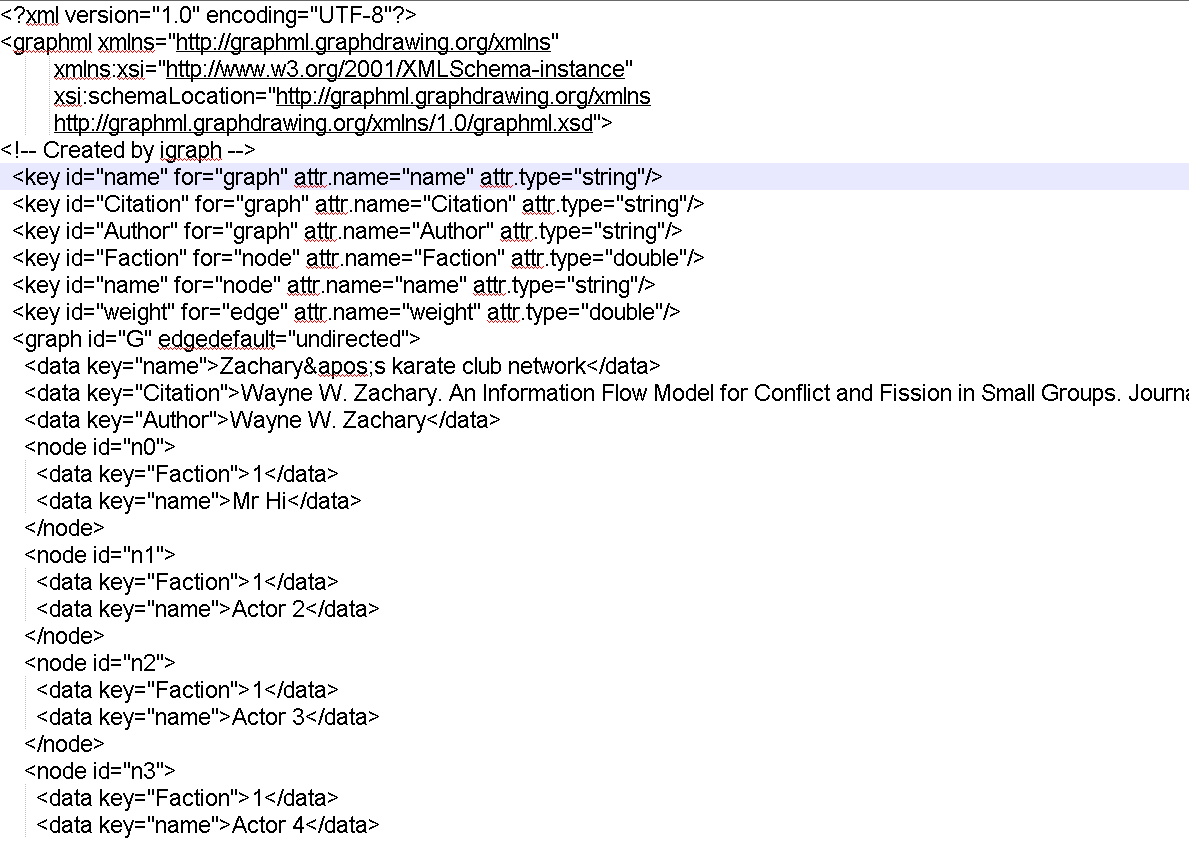
\includegraphics[scale=0.6]{input.png}
        \caption{Sample Karate GraphML file}
        \label{g1}
    \end{center}
\end{figure}
\newpage
\subsubsection{Graph before splitting into 2 clusters}
\begin{figure}[ht]    
    \begin{center}
        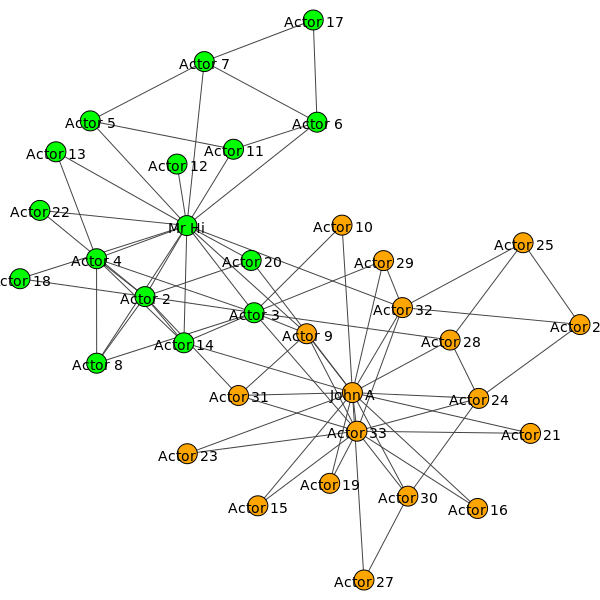
\includegraphics[scale=0.7]{group1.png}
        \caption{Original Graph}
        \label{g2}
    \end{center}
\end{figure}
\newpage
\subsubsection{Command line output of nodes in each cluster and number of edges deleted to get 2 clusters}
\begin{figure}[ht]    
    \begin{center}
        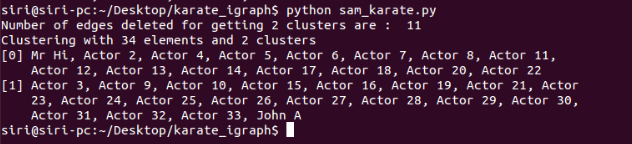
\includegraphics[scale=1.0]{cmd_1.png}
        \caption{Command line output}
        \label{g3}
    \end{center}
\end{figure}
\subsubsection{Graph after splitting into 2 clusters}
\begin{figure}[ht]    
    \begin{center}
        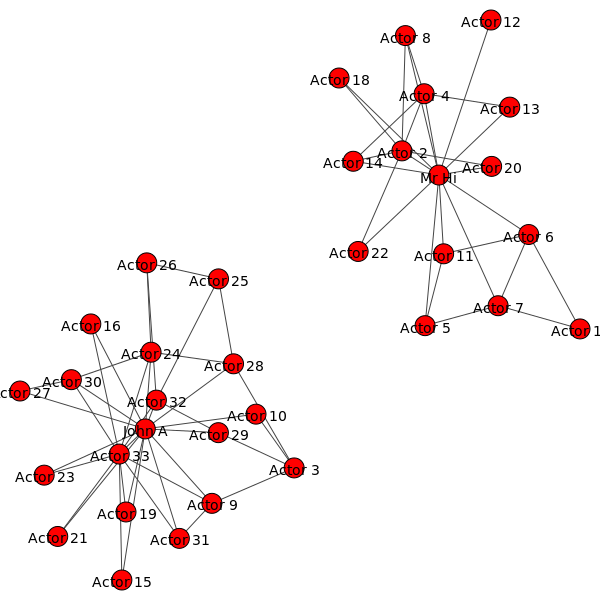
\includegraphics[scale=0.5]{output1.png}
         \caption{Predicted Graph}
        \label{g4}
    \end{center}
\end{figure}
\newpage

\subsection{Conclusion}
\begin{enumerate}
\item The initial graph which can be seen in figure\ref{g2} is represented in 2 colors.
\item All the actors in green belong to Mr. Hi group and all the actors in orange belong to John's group.
\item This graph is drawn based on the ``Faction'' key in the graphML which groups all the actors into Mr. Hi's group or John's group.
\item Output graph of 2 clusters can be seen here in figure\ref{g4}.
\item Now when I compare both of these, we can observe that ``Actor 3'' is in Mr. Hi's group, this is according to the Faction key which is the original graph.
\item Whereas, In the predicted graph that we got by implementing the Girvan-Newman Algorithm, ``Actor 3'' is in John's group.
\item So, Except Actor 3 all other predictions are correct and this proves that the predicted graph is highly accurate. 
\item Finally, this solution tells us that Girvan-Newman Algorithm produces predicted graphs accurately.

\end{enumerate}
